\section{Oscilador Harmônico Amortecido}

\subsection{Conceitos}
O oscilador harmônico amortecido descreve o movimento mecânico de um oscilador (ex: pêndulo de massa-mola) sob a influência de uma força restauradora e atrito. O movimento do pêndulo depende basicamente de 3 forças:

\begin{itemize}	
\item Força de inércia $F = m \, \ddot{x}$
\item Força restauradora $F_{f} = -kx$
\item Força de amortecimento $F_{r} = -\mu \, \dot{x}$
\end{itemize}

\begin{figure}[H]
	\centering
	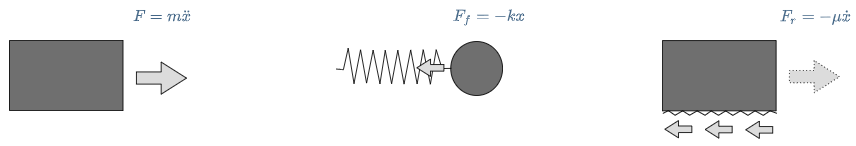
\includegraphics[width=0.8\textwidth]{./Imagens/Oscilador/OH1.png} 
	\caption{Tipos de forças atuantes}
	\label{fig:OH1}
\end{figure}

\subsection{Força de inércia}
Advém da 2° Lei de Newton que diz que a força resultante que atua sobre um corpo é igual ao produto de sua massa pela aceleração.

\subsection{Força restauradora}
É a força que puxa a massa do pêndulo de volta para sua posição de repouso. Esta força é diretamente proporcional ao deslocamento em relação à posição de equilíbrio.

\begin{itemize} 
\item $x$: é o deslocamento da posição de equilíbrio, em metros (m).
\item $k$: é a constante de proporcionalidade, dada por $\large \frac{mg}{L}$ e que depende do material.
\end{itemize}

\subsection{Força de amortecimento}
É a força de resistência ao movimento relativo entre superfícies sólidas, camadas de fluidos e outros materiais que deslizam um contra o outro. Essa força de atrito é proporcional à velocidade do pêndulo.
\begin{itemize}
\item $\dot{x}$:  velocidade de deslocamento de uma massa em relação a um ponto fixo.
\item $\mu$: é o coeficiente de atrito que depende do material e da forma da matéria
\end{itemize}

\subsection{Equação do movimento}

A força resultante será a soma da força restauradora e de amortecimento.

\begin{equation}
\large m \ddot{x} = -\mu \dot{x} -kx \rightarrow \ddot{x} + \frac{\mu}{m}\dot{x} + \frac{k}{m}x = 0
\tag{6.1}
\end{equation}
	
Esta equação é uma equação diferencial linear, homogênea, de segunda ordem e com coeficientes constantes. 

\begin{itemize}

\item Vamos definir $\large \omega _{0} = \sqrt{\frac{k}{m}}$ como a frequência natural de vibração não amortecida do sistema.

\item Vamos definir a sigla $\zeta$ como o \textbf{coeficiente de amortecimento} ou simplesmente \textbf{amortecimento}, sendo a sua fórmula:

\begin{equation}
\large \zeta = \frac{\mu}{2\sqrt{km}} 
\tag{6.2}
\end{equation}

\item Vamos considerar ainda $\large p = \frac{dx}{dt}$.

\end{itemize}

A equação do movimento, fica, então:

\begin{equation}
\large \frac{dp}{dt} = -2\zeta w_{0} p - w_{0}^2x 
\tag{6.3}
\end{equation}

O termo $-2\zeta w_{0}$ é responsável pelo amortecimento. Caso o coeficiente de amortecimento $-2\zeta w_{0}$ seja nulo, o sistema passa a oscilar indefinidamente, realizando um \textbf{Movimento Harmônico Simples (MHS)}.

\subsection{Amortecimento}

\begin{itemize}
	
\item O amortecimento é uma influência dentro ou sobre um sistema oscilatório que tem o efeito de reduzir, restringir ou prevenir suas oscilações.
 
\item O \textbf{coeficiente de amortecimento} é uma medida adimensional que descreve como as oscilações em um sistema decaem após uma perturbação. Muitos sistemas exibem comportamento oscilatório quando são perturbados de sua posição de equilíbrio estático.

\item Uma massa suspensa por uma mola pode, se puxada e liberada, pular para cima e para baixo. O sistema tende a retornar à sua posição de equilíbrio a cada salto, mas a ultrapassa. Às vezes, as perdas (por exemplo, atrito) amortecem o sistema e podem fazer com que as oscilações diminuam gradualmente em amplitude para zero ou se atenuem. O \textbf{coeficiente de amortecimento} é uma medida que descreve a rapidez com que as oscilações diminuem de um salto para o outro. 

\end{itemize}

\subsubsection{Fórmula do amortecimento}

O coeficiente de amortecimento é geralmente representado pela sigla $\zeta$ e sua fórmula é:

\begin{equation}
\large \zeta = \frac{\mu}{2\sqrt{km}}
\tag{6.4}
\end{equation}

\subsubsection{Tipos de amortecimento}

O coeficiente de amortecimento ($\zeta$) fornece indicações de como será a resposta transitória do sistema:

\begin{itemize}
\item Se $\zeta > 1$: sistema superamortecido (overdamped). O sistema retorna (decai exponencialmente) para o estado estável sem oscilar.
\item Se $\zeta = 1$: sistema criticamente amortecido (critically damped). O sistema retorna para o estado estável rapidamente e sem oscilar.
\item Se $0 < \zeta < 1$: sistema subamortecido (underdamped).  O sistema oscila com uma freqüência levemente diferente que o do caso não amortecido com a amplitude gradualmente decrescendo a zero.
\item Se $\zeta = 0$: sistema não amortecido. O sistema oscila sem perda de amplitude.

\end{itemize}


\subsection{Oscilador harmônico amortecido no Python}

O gráfico da posição vs tempo de um oscilador harmônico foi obtido com o uso da biblioteca \textbf{odeint} do Python, que possibilita o usuário a encontrar as soluções de um sistema de equações diferenciais ordinárias.

\begin{minted}{python}
from scipy . integrate import odeint
import numpy as np
from matplotlib import pyplot as plt

def dy(y, t, zeta, w0):
x, p = y[0], y[1]
dx = p
dp = -2 * zeta * w0 * p - w0**2 * x
return [dx, dp]

# estado inicial
y0 = [1.0, 0.0]

# intervalo de tempo
t = np.linspace(0, 10, 1000)
w0 = 2*np.pi*1.0 # frequência natural
# print(w0)

# resolvendo a EDO para 4 diferentes 
# valores de amortecimento
# não amortecido
y1 = odeint(dy, y0, t, args=(0.0, w0)) 
# sub-amortecido
y2 = odeint(dy, y0, t, args=(0.2, w0))
# criticamente amortecido 
y3 = odeint(dy, y0, t, args=(1.0, w0)) 
# super-amortecido
y4 = odeint(dy, y0, t, args=(5.0, w0)) 

fig, ax = plt.subplots(figsize = (10,8))
ax.plot(t, y1[:,0], 'k', label="não amortecido", 
linewidth=0.5)
ax.plot(t, y2[:,0], 'r', label="sub-amortecido")
ax.plot(t, y3[:,0], 'b', label=r"criticamente amortecido")
ax.plot(t, y4[:,0], 'g', label="super-amortecido")
ax.legend()
plt.show()
\end{minted}

\begin{figure}[H]
	\centering
	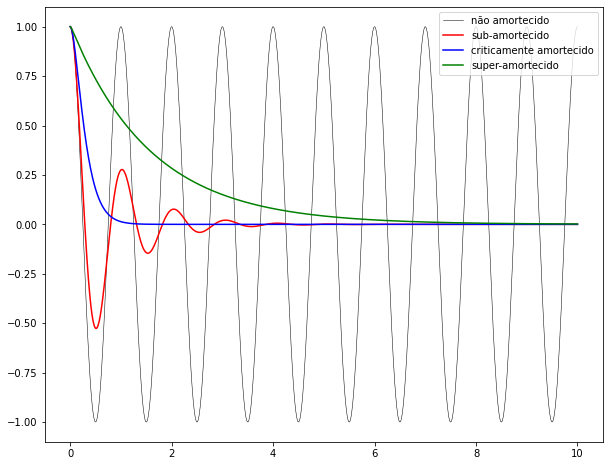
\includegraphics[width=0.8\textwidth]{./Imagens/Oscilador/OH2.png} 
	\caption{Gráfico posição x tempo}
	\label{fig:OH2}
\end{figure}

\subsection{Aplicações da oscilação harmônica amortecida}

\begin{itemize}
\item Em sistemas físicos, o amortecimento é produzido por processos que dissipam a energia armazenada na oscilação. Os exemplos incluem arrasto viscoso em sistemas mecânicos, resistência em osciladores eletrônicos e absorção e dispersão de luz em osciladores ópticos. 
\item Na engenharia elétrica, as repostas naturais de circuitos RLC podem ser super-amortecido, criticamente amortecido, sub-amortecido ou sem amortecimento.
\item Os amortecedores de um carro amortecem criticamente a suspensão do veículo e, portanto, resistem à vibrações que poderiam dificultar o controle ou causar danos. 
\item Amortecedores de porta evitam que a porta oscile quando ela é fechada graças à esse princípio.
\end{itemize}